%%%%%%%%%%%%%%%%%%%%%%%%%%%%%%%%%%%%%%%%%%%%%%%%%%%%%%%%%%%%%%%%%%%%%%%%%%%%%%%%
% results.tex:  
%%%%%%%%%%%%%%%%%%%%%%%%%%%%%%%%%%%%%%%%%%%%%%%%%%%%%%%%%%%%%%%%%%%%%%%%%%%%%%%%
\chapter{Results}
\label{results}

The events in the partial disappearance region and the tag/probe invariant mass distribution for events in the complete disappearance region are shown in \Cref{fig:invMassResult} for the observed data and estimated backgrounds.

\begin{figure}[htbp]
	\centering
	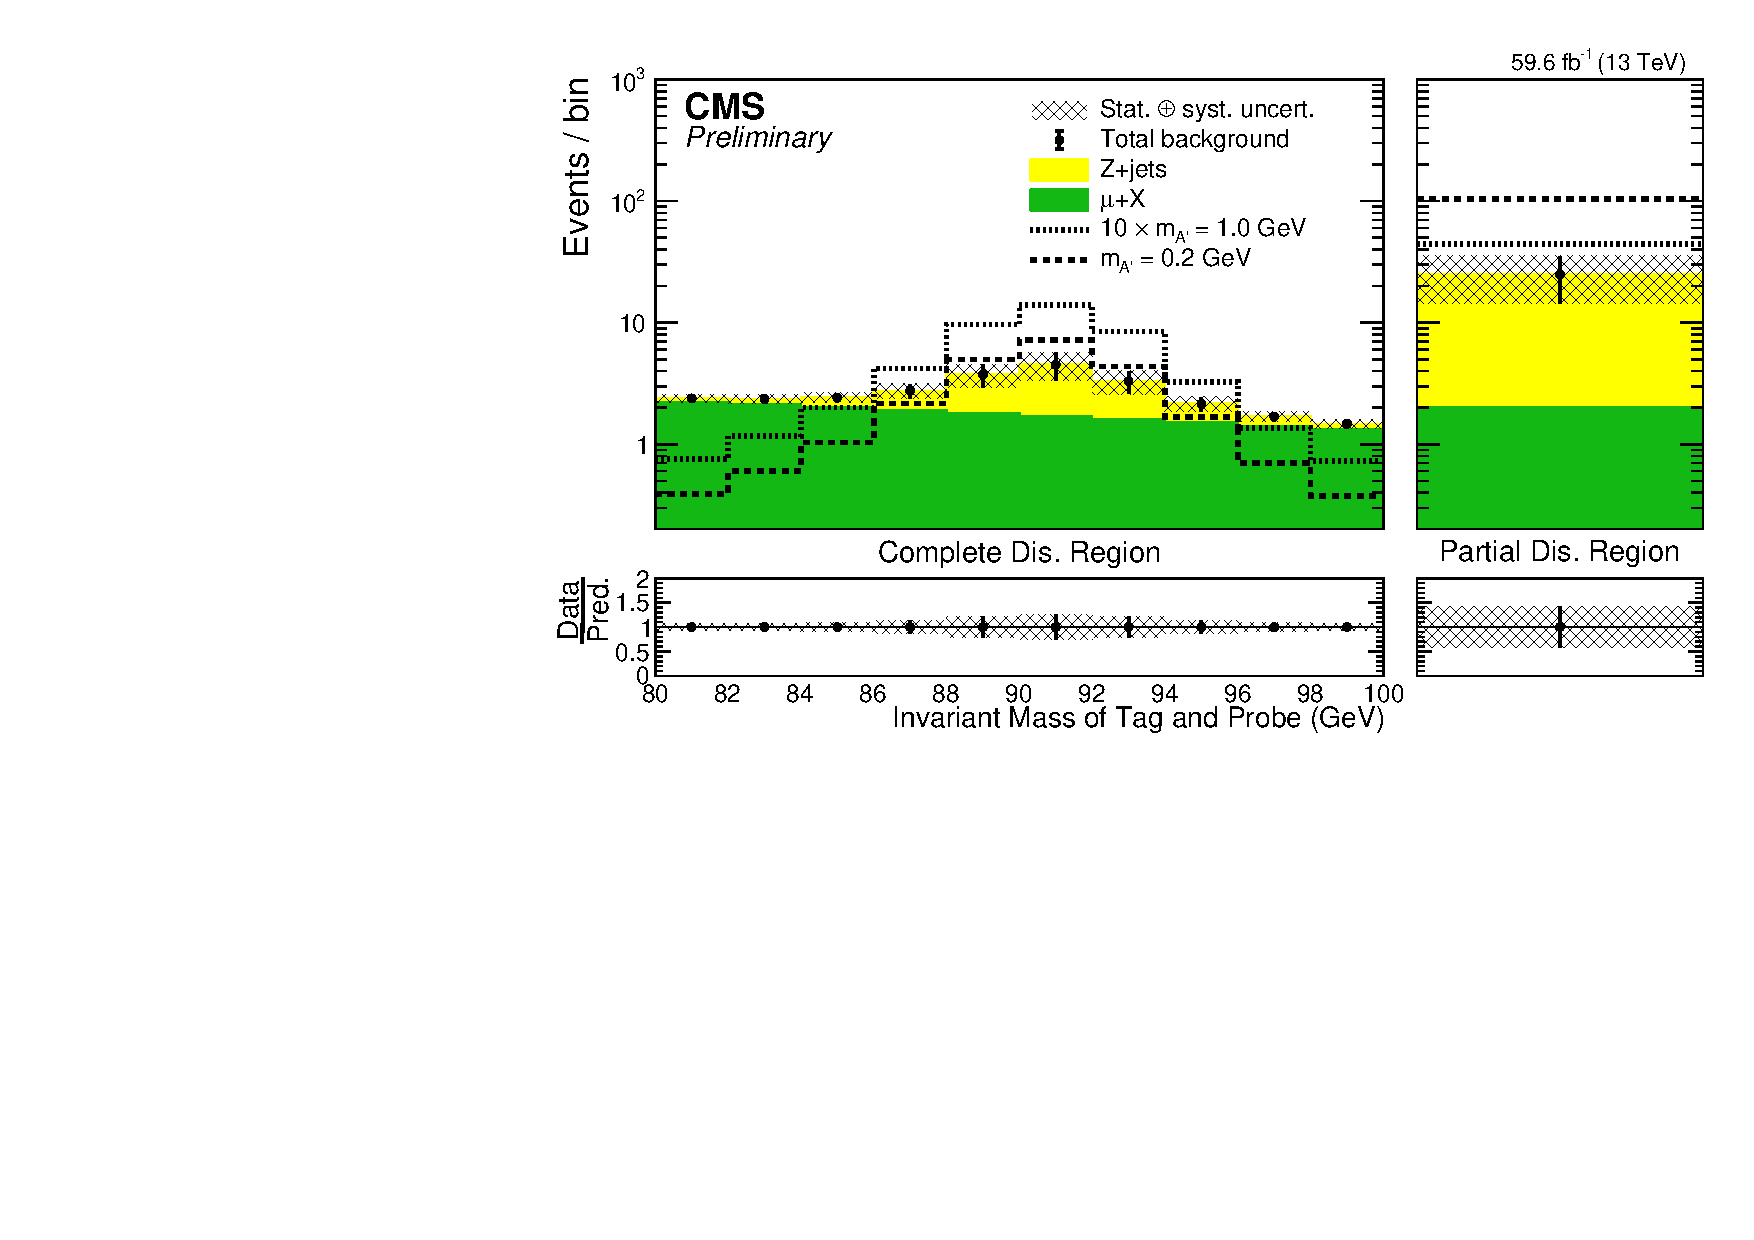
\includegraphics[width=0.8\textwidth]{figures/bdtScore_partialDisappearanceBDT_0p2.pdf}
	\caption[Observed Signal Region Events]{The di-muon invariant mass of complete disappearance events and the number of partial disappearance events seen in data, as well as the predicted backgrounds from simulation and the off-peak control region.}
	\label{fig:invMassResult}
\end{figure}

The results are combined with the measured fixed target luminosities from the signal simulation in order to interpret them as limits on the square of the mixing paramer, which the \dbrem interaction rate is directly proportional to.
The obtained upper limits are presented in \Cref{fig:limits} as a function of the dark photon mass. 

\begin{figure}[htbp]
	\centering
	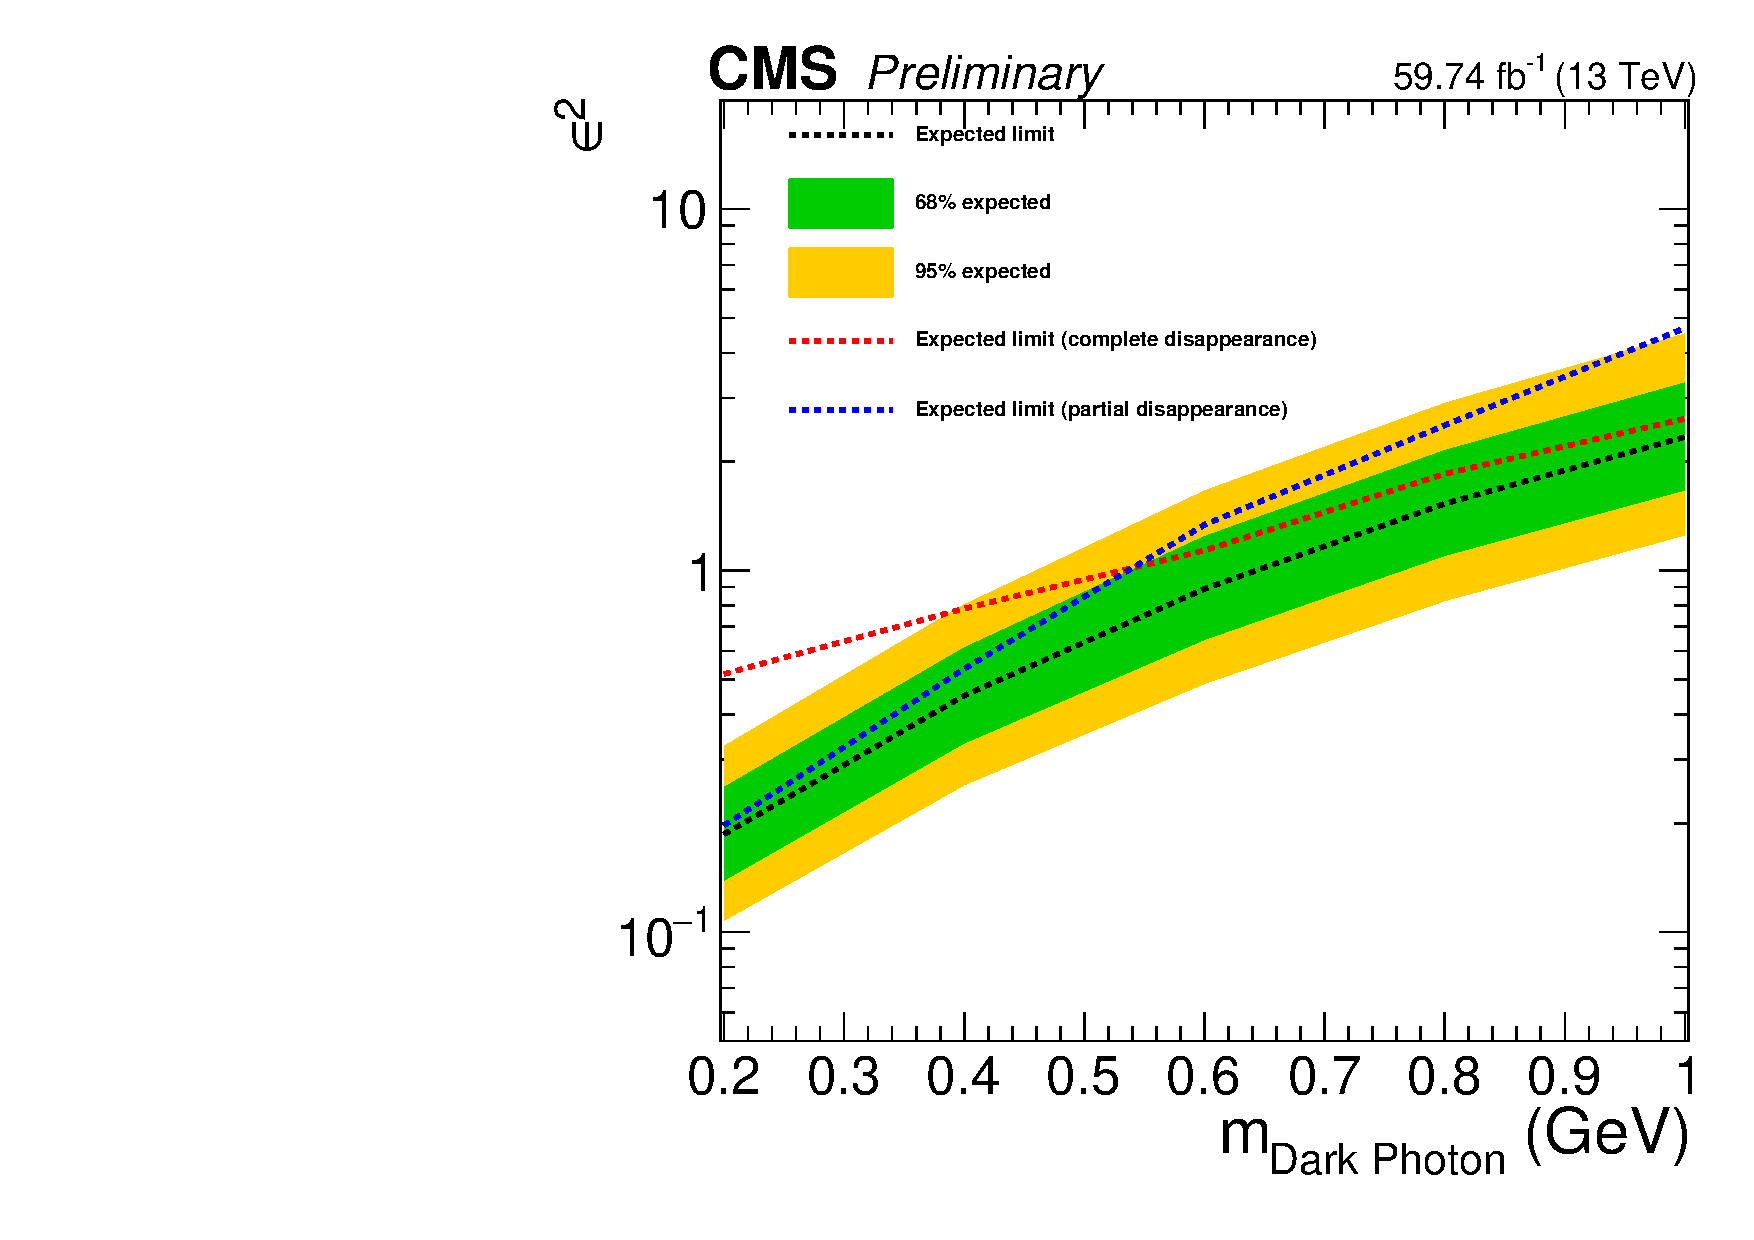
\includegraphics[width=0.8\textwidth]{figures/Limit_AllRegions.pdf}
	\caption[Exclusion Limits on the Dark Photon Mixing Parameter]{The exclusion limit for the square of the dark photon mixing parameter as a function of the A' mass.}
	\label{fig:limits}
\end{figure}

At lower masses the partial disappearance region dominates, as the lighter mass dark photons tend to have higher energy outgoing muons, while the complete disappearance region is stronger for larger A' masses. 
The decreasing cross section with dark photon mass decreases the interaction rate more quickly than the relative increase in selection efficiency created by the lower energy outgoing muons at large A' mass, resulting in stronger exclusion limits at small mediator masses. 
In cases where the dark photon mass becomes comparible to the muon mass ($\sim$0.1 GeV), the \ww approximation used to calculate the interaction probability breaks down, and so these points are not included in the produced limits.

